\clearpage\section{Entrega 02: Método Simbólico, Análisis Combinatorio, Titulares de Fake News}
\section*{Problema 1: Método Simbólico}
En el análisis combinatorio existe un método que permite la definición formal de estructuras combinatorias a partir de sus propiedades. Este método se conoce como el método simbólico. Este método provee definiciones básicas que permiten definir estructuras combinatorias, y que a través de esta definición y el \textit{teorema de transferencia}, se permite obtener la respectiva \textbf{función generadora} y así, una fórmula para las estructuras.

Este método está basado primeramente en la definición de \textit{clases combinatorias}. Por ejemplo, $\mathcal{B}$ se podría definir como la clase combinatoria de todas las cadenas binarias. Adicional a esta definición, se requiere de la definición de átomo, que corresponde a los elementos que conforman la clase combinatoria. En el caso de las cadenas binarias, está conformado por los caracteres $0$ y $1$, y en el método simbólico, serían definidos como $z_0$ y $z_1$. Por último está la definición del elemento nulo o vacío, $\epsilon$.

\begin{table}[h!]
    \centering
    \begin{tabular}{|c|c|c|}
    \hline
        Definición &  Método Simbólico & Función Generadora\\
    \hline
        Clase Combinatoria & $\mathcal{A}$ &  $A(z)$\\
    \hline
        Átomo & $z_0,\,z_1,\,z_2,\,\dots$ & $z$ \\
    \hline 
        Vacío & $\epsilon$ & $1$ \\
    \hline
        Unión  & $\mathcal{A} + \mathcal{B}$ & $A(z) + B(z)$\\
    \hline
        Pares Ordenados & $\mathcal{A}\times\mathcal{B}$ & $A(z)\cdot B(z)$\\
    \hline
        Secuencia &  $SEQ(\mathcal{A})$ & $\cfrac{1}{1-A(z)}$\\
    \hline
    \end{tabular}
    \caption{Método Simbólico}
    \label{tab:sym_method}
\end{table}

\begin{itemize}
    \item Los átomos son las unidades básicas de la clase combinatoria.
    \item $\mathcal{A} + \mathcal{B}$ es la clase que contiene copias disyuntas de los miembros de $\mathcal{A}$ y $\mathcal{B}$. 
    \item $\mathcal{A} \times \mathcal{B}$ es la clase de pares ordenados (producto cartesiano) de $\mathcal{A}$ y $\mathcal{B}$.
\end{itemize}

\section*{Ejemplos}

\paragraph{Ejemplo 1}
Aplique el método simbólico para determinar el número total de cadenas ternarias de longitud $n$.

1. \textbf{Clase combinatoria}.
$\mathcal{T}$ es la clase combinatoria de las cadenas ternarias de longitud $n$.

2. \textbf{Átomos}.
Dado que las cadenas ternarias están conformadas por los caracteres $0$, $1$ y $2$, definimos los átomos $z_0,\,z_1$ y $z_2$.

3. \textbf{Construcción combinatoria}.
Las cadenas ternarias se pueden definir como los átomos (0, 1 y 2), unidos a una cadena ternaria. Y en efecto, mediante la sucesiva unión de 0, 1 y 2, se pueden obtener todas las cadenas ternarias.

\begin{equation*}
    \mathcal{T} = \epsilon + (z_0 + z_1 + z_2) \times \mathcal{T}.
\end{equation*}

{\color{magenta} Nótese que en caso de que no se incluyera el elemento vacío, la clase combinatoria no estaría generando nada, dado que los átomos se le están adjuntando a elementos de la clase ya generados.}

4. \textbf{Transformación a funciones generadoras.}

Esto se hace por medio de la aplicación de lo establecido en la tabla \ref{tab:sym_method}.
\begin{equation*}
\begin{split}
    T(z) &= 1 + (z + z + z)\cdot T(z)\\
    T(z) &= 1 + 3z\cdot T(z)\\
    T(z)[1 - 3z] &= 1\\
    T(z) &= \cfrac{1}{1-3z}.
\end{split}
\end{equation*}
5. \textbf{Transformación a secuencia f(n).}

De la tabla de funciones generadoras básicas se sabe que
\begin{align*}
    T(z) &= \sum_{^n\ge 0}f(n)\cdot z^n\\
    T(z) &=\cfrac{1}{1-3z}=\sum_{^n\ge 0}3^n\cdot z^n\\
    &\to \boxed{f(n)=3^n}
\end{align*}

Por tanto, se obtiene que el número de cadenas ternarias de longitud $n$ es $3^n$.

\paragraph{Ejemplo 2.}
Ahora resolveremos el mismo ejercicio, pero de un modo un poco diferente.

1. \textbf{Clase combinatoria}.
$\mathcal{T}$ es la clase combinatoria de las cadenas ternarias.

2. \textbf{Átomos}.
Dado que las cadenas ternarias están conformadas por los caracteres $0$, $1$ y $2$, definimos los átomos $z_0,\,z_1$ y $z_2$.

3. \textbf{Construcción combinatoria}.
Las cadenas ternarias también pueden ser vistos como una \textit{secuencia} de ceros, unos y dos. Esto es:
\begin{equation*}
    \mathcal{T} = SEQ(z_0 + z_1 + z_2).
\end{equation*}
{\color{magenta} Aquí no se incluye el elemento vacío, porque la misma secuencia lo incluye.}

4. \textbf{Transformación a funciones generadoras}
\begin{equation*}
\begin{split}
    T(z) &= \frac{1}{1-(z + z + z)}\\
    T(z) &= \cfrac{1}{1-3z}
\end{split}
\end{equation*}
5. \textbf{Transformación a secuencia f(n).}

Se procede de igual forma que el ejemplo anterior.

\paragraph{Ejemplo 3.}
Cadenas binarias que No contienen la subcadena \texttt{11}.

1. \textbf{Clase combinatoria}.
$\mathcal{B}_{\overline{11}}$: Cadenas binarias que no contienen la subcadena \texttt{11}.

2. \textbf{Átomos}.
$$z_0,\,z_1$$
3. \textbf{Construcción combinatoria}.

Basados en el diseño (árbol binario), 
$$\mathcal{B}_{\overline{11}} = \epsilon  + z_0 + (z_1 + z_0\times z_1)\times\mathcal{B}_{\overline{11}}$$

Al añadir $z_1$ delante de $z_0$, se evita que hayan 2 unos consecutivos, dado que estará siempre seguido de por lo menos un 0, a excepción del caso donde solo hay un 1, que como se ve, está incluido aparte.

4. \textbf{Transformación a funciones generadoras}
\begin{equation*}
\begin{split}
   B(z) &= 1 + z + (z + z^2)\cdot B(z)\\
   B(z)[1 - z - z^2] &= 1 + z\\
   B(z) &= \cfrac{1+z}{1-z-z^2}\\
   B(z) &= \cfrac{1}{1-z-z^2}+\cfrac{z}{1-z-z^2}
\end{split}
\end{equation*}
5. \textbf{Transformación a secuencia f(n).}

En clase mostramos que la FGO $\cfrac{1}{1-z-z^2}$ genera la secuencia $f(n)=Fib(n)$ \\\\
Entonces:
$B(z)$ genera $f(n)=Fib(n)+Fib(n-1)=Fib(n+1)$, donde $Fib(n)$ es el $n$-ésimo número de Fibonacci.\\

Para más información sobre este método, se recomienda consultar \cite{sedgewick_introduction_2013}, \cite{lehman_generating_2010} y \cite{sedg-symb}.\\

\clearpage
Para los siguientes problemas debe definir la respectiva expresión mediante el método simbólico, obtener la función generadora, y sacar sus coeficientes. Adicionalmente, debe crear un programa en Python que a través de un menú, permita seleccionar cualquiera de estas opciones y dado un valor de $n$, mostrar {\color{cyan} cuántas y cuáles} cadenas de longitud $n$ cumplen con la condición pedida. {\color{red} El programa \textbf{no puede} generar todas las cadenas de longitud $n$ y de estas, eliminar las que no cumplan}.


\begin{enumerate}
    \item \,[*] Cadenas Binarias, de longitud n, que:
    \begin{itemize}
        \item Contengan la subcadena '10'\\
        1.\textbf{Clase combinatoria:}Cadenas binarias que contienen la subcadena $10$\\
        2.\textbf{Átomos:} $z_0, z_1$\\
        3.\textbf{Construcción combinatoria:}\\
        \begin{align*}
            B(z) &= \epsilon + (z_0+z_1)\cdot B(z)\\
        \end{align*}\\
        4.\textbf{Transformación a funciones generadoras:}
        \begin{align*}
            B(z) &= \epsilon + (z_0+z_1)\cdot B(z)\\
            B(z) &= 2z\cdot B(z)+z^2\cdot (S(z)-B(z))\\
            B(z)\cdot (1-2z+z^2) &= \frac{z^2}{1-2z}\\
            B(z) &= \frac{z^2}{(1-2z)(1-2z-z^2)}
        \end{align*}
        (Estudiante: Alejandra Landinez - 200161946)\\
        \item Que No contengan '010'\\
        \textbf{Créditos:} Profe Alfonso Mancilla\\
        1.\textbf{Clase combinatoria:}Cadenas binarias que no contienen la subcadena $010$\\
        2.\textbf{Átomos:} $z_0, z_1$\\
        3.\textbf{Construcción combinatoria:}\\
        \begin{align*}
            B(z) &= z_1\cdot B(z)+SEQ(z_0)+(\epsilon+z_0\cdot z_1\cdot \epsilon +z_0\cdot z_1\cdotB(z)
        \end{align*}\\
        4.\textbf{Transformación a funciones generadoras:}\\
        \begin{align*}
            B(z) &= z_1\cdot B(z)+SEQ(z_0)+(\epsilon+z_0\cdot z_1\cdot \epsilon +z_0\cdot z_1\cdotB(z)\\
            B(z)\cdot \left(\frac{1-z-z^2}{1-z}\right)&= \frac{1+z^2}{1-z}\\
            B(z)\cdot(1-2z+z^2-z^3) &= (1+z^2)\\
            B(z) &= \frac{1+z^2}{1-2z+z^2-z^3}
        \end{align*}\\
        \end{itemize}
    \item \,[*] Cadenas Ternarias, de longitud n, que:
    \begin{itemize}
        \item No contengan la subcadena '12'\\
        \textbf{Créditos:} Profe Alfonso Mancilla\\
        1.\textbf{Clase combinatoria:}Cadenas ternarias que no contienen la subcadena $12$\\
        2.\textbf{Átomos:} $z_0, z_1, z_2$\\
        3.\textbf{Construcción combinatoria:}\\
        \begin{align*}
            T(z) &= (z_0+z_2)\cdot T(z)+SEQ(z_1)\cdot (\epsilon+z_1\cdot z_0\cdot T(z)
        \end{align*}\\
        4.\textbf{Transformación a funciones generadoras:}\\
        \begin{align*}
            T(z) &= (z_0+z_2)\cdot T(z)+SEQ(z_1)\cdot (\epsilon+z_1\cdot z_0\cdot T(z)\\
            T(z) &= 2z\cdot T(z)+\frac{(1+z^2\cdot T(z))}{1-z}\\
            T(z)\cdot\left[\frac{1+z^2\cdot T(z)}{1-z}\right]&= \frac{1}{1-z}\\
            T(z)\cdot\left[1+2z^2-3z-z^2\right] &= 1\\
            T(z) &= \frac{1}{1-3z+z^2}
        \end{align*}\\
        (Estudiante: Alejandra Landinez - 200161946)\\
        \item Que contengan la subcadena '012'\\
        \textbf{Créditos:} Profe Alfonso Mancilla
        1.\textbf{Clase combinatoria:}Cadenas ternarias que contienen la subcadena $012$\\
        2.\textbf{Átomos:} $z_0, z_1, z_2$\\
        3.\textbf{Construcción combinatoria:}\\
        \begin{align*}
            T(z) &= \epsilon + (z_0+z_1+z_2)\cdot T(z)\\
        \end{align*}\\
        4.\textbf{Transformación a funciones generadoras:}\\
        \begin{align*}
            T(z) &= \epsilon + (z_0+z_1+z_2)\cdot T(z)\\
            T(z) &= 3z\cdot T(z)+z^3\cdot (S(z)-T(z))\\
            T(z)\cdot (1-3z+z^3) &= \frac{z^3}{1-3z}\\
            T(z) &= \frac{z^3}{(1-3z)(1-3z-z^3)}
        \end{align*}\\
        \item Que contengan un número par de unos\\
         1.\textbf{Clase combinatoria:}Cadenas ternarias que contienen un número par de unos\\
        2.\textbf{Átomos:} $z_0, z_1, z_2$\\
        3.\textbf{Construcción combinatoria:}\\
        \begin{align*}
            T(z) &= \epsilon + (z_0+z_1+z_2)\cdot T(z)
        \end{align*}\\
         4.\textbf{Transformación a funciones generadoras:}\\
        \begin{align*}
            T(z) &= \epsilon + (z_0+z_1+z_2)\cdot T(z)\\
            T(z) &= 1+ 3z\cdot T(z)\\
            T(z) &= T(z)\cdot 3z+1\\
            T(z)\cdot(1-3z) &= 1 \\
            T(z) &= \frac{1}{1 - 3z}
        \end{align*}\\
        (Estudiante: Alejandra Landinez - 200161946)
        \end{itemize}     
\item \,[*] Cadenas numéricas, de longitud n, de base cinco que:
    \begin{itemize}
        \item Tengan sus caracteres en orden creciente. Ejemplo '01122234'\\
        \textbf{Créditos:} Profe Alfonso Mancilla\\
        1.\textbf{Clase combinatoria:}Cadenas numéricas de base cinco que contienen sus caracteres en orden creciente\\
        2.\textbf{Átomos:} $z_0, z_1, z_2, z_3, z_4$\\
        3.\textbf{Construcción combinatoria:}\\
        \begin{align*}
            Q(z) &= SEQ(z_0)\cdot SEQ(z_1)\cdot SEQ(z_2)\cdot SEQ(z_3)\cdot SEQ(z_4)
        \end{align*}
        4.\textbf{Transformación a funciones generadoras:}\\
        \begin{align*}
            Q(z) &= SEQ(z_0)\cdot SEQ(z_1)\cdot SEQ(z_2)\cdot SEQ(z_3)\cdot SEQ(z_4)\\
            Q(z) &= \left[\frac{1}{1-z}\right]^5\\
            Q(z) &= \binom{n+5-1}{5}
        \end{align*}
        \item Que No contengan las subcadenas '01' ni '43' 
    \end{itemize}
\end{enumerate}
\section*{Problema 2: Conteo mediante funciones generadoras ordinarias}
	
Las funciones generadoras ordinarias (FGO) nos permiten resolver problemas relacionados con conteo, de una manera sencilla; de modo que mediante manipulaciones sencillas sobre estas, problemas que sería difícil resolver directamente, son resueltos por medio de operaciones mucho más simples como la suma de polinomios o la multiplicación de estos.
	
Recordemos que la función generadora $F(z)$ de una secuencia $f_n$ es de la forma
	
$$F(z)=\sum_{n\geq0}{f_n\cdot z^n}$$
	
Es importante tener en cuenta que de aquí en adelante $f_n$ siempre hace referencia al número de conjuntos de $n$ objetos idénticos.
	
En esta sección se mostrará que este $f_n$ puede ser asociado a un problema de conteo y que por medio de el uso de FGO, se puede hallar con facilidad una expresión cerrada para $f_n$. En estos problemas, obtendremos la FGO de $f_n$ y luego hallaremos el coeficiente de esta función generadora. Es decir, a a partir de $F(z)$ hallaremos $f_n$. Recordemos la notación $[z^n]F(z)=f_n$.
	
En este  tipo de ejercicios, las siguientes funciones generadoras suelen ser bastante comunes, por lo que es muy importante tenerlas presentes:
\begin{align*}
[z^n]\cfrac{1}{(1-z)^m}&=\binom{m+n-1}{n}\\
[z^n]\cfrac{z^{m}}{(1-z)^{m+1}}&=\binom{n}{m}\\
\end{align*}
Veamos algunos ejemplos.

\paragraph{Ejemplo 1}
Sea $f_n$ el número de maneras de $\textbf{seleccionar}$ $n$ pelotas a partir de infinitas pelotas verdes, azules y doradas.

Es posible plantear el problema como una ecuación entera, de tal modo que $f_n$ sea el número de soluciones a esta ecuación. En este caso, es:

$$S_{\rm v}+S_{\rm a} + S_{\rm d}=n,\quad 0\leq S_{\rm v},\,S_{\rm a},\,S_{\rm d}.$$
Donde $S_{\rm v}$ representa el número de pelotas verdes, $S_{\rm a}$  representa el número de pelotas azules y $S_{\rm d}$ representa el número de pelotas doradas. Claramente, no puede haber un número de pelotas negativo. La ecuación dicta que la suma de la cantidad de pelotas debe ser igual a $n$, en este caso, sin restricciones, tal como indica la definición de $f_n$.

Este problema puede plantearse de la siguiente manera, sin recurrir a funciones generadoras:
$$f_n=\sum_{S_{\rm v}+S_{\rm a} + S_{\rm d}=n}{1},$$
sin embargo, al aproximarnos a la solución utilizando funciones generadoras, el proceso será más sencillo que si se tratara de empezar utilizando esta expresión.

\subsubsection*{Solución mediante FGO}
La solución a este tipo de problemas mediante FGO consiste en los siguientes pasos:

\begin{enumerate}
	\item El primer paso a realizar es \textbf{modelar el problema como una ecuación entera, incluyendo las restricciones}. 
	\item El segundo paso a realizar es el de plantear la función generadora $F(z)$ para $f_n$ a partir de la ecuación planteada.
	\item Finalmente, se procede a hallar el coeficiente de $F(z)$, que al ser la función generadora definida a partir del problema, equivale a una \textbf{expresión cerrada} para $f_n$.
\end{enumerate}


Sea $f_n\equiv$ el número de maneras de $\textbf{seleccionar}$ $n$ pelotas a partir de infinitas pelotas verdes, azules y doradas, entonces la ecuación que modela este problema es

$$S_{\rm v}+S_{\rm a} + S_{\rm d}=n,\quad 0\leq S_{\rm v},\,S_{\rm a},\,S_{\rm d}.$$

Una vez se ha modelado el problema como una ecuación entera, definimos $F(z)$ como la función generadora de $f_n$ y la expresamos a partir de la ecuación planteada. Esto es:

$$F(z)=\left(\sum_{S_{\rm v}\geq 0} {z^{S_{\rm v}}}\right)\cdot\left(\sum_{S_{\rm a}\geq 0} {z^{S_{\rm a}}}\right)\cdot\left(\sum_{S_{\rm d}\geq 0} {z^{S_{\rm d}}}\right).$$

En este caso usamos las mismas variables usadas en la ecuación, pero también es posible usar la letra $n$:
$$F(z)=\underbset{S_{\rm v}}{\left(\sum_{n\geq 0} {z^{n}}\right)}\cdot\underbset{S_{\rm a}}{\left(\sum_{n\geq 0} {z^{n}}\right)}\cdot\underbset{S_{\rm d}}{\left(\sum_{n\geq 0} {z^{n}}\right)}.$$
La elección es cuestión de preferencia. Pero es importante, en cualquiera de los dos casos, señalar a qué variable de la ecuación corresponde cada sumatoria.

Una vez planteada la función generadora de $f_n$, $F(z)$, pasamos a hacer uso de las FGO básicas. En este caso, sabemos que
$\sum_{n\geq0}z^n=\cfrac{1}{1-z}$, por lo tanto:
\begin{align*}
F(z)&=\left(\sum_{n\geq 0} {z^{n}}\right)\cdot
\left(\sum_{n\geq 0} {z^{n}}\right)\cdot\left(\sum_{n\geq 0} {z^{n}}\right)\\
&=\left(\cmag{\sum_{n\geq 0} {z^{n}}}\right)^3
=\left(\cmag{\cfrac{1}{1-z}}\right)^3.
\end{align*}
Aquí, hemos llegado a que
$$F(z)=\cfrac{1}{(1-z)^3}.$$

Una vez llegamos a una expresión de este tipo para $F(z)$, el siguiente paso es hallar el coeficiente $f_n$ de esta expresión. Aquí, nuevamente recurrimos a la tabla de FGO básicas.
Y recordemos que
\begin{align*}
[z^n]\cfrac{1}{(1-z)^m}&=\binom{m+n-1}{n},
\end{align*}
es decir, el coeficiente de FGO de esta forma es $\binom{m+n-1}{n}$. Aplicando esto a este ejemplo, con $m=3$, tenemos que:
$[z^n]F(z)=\binom{3+n-1}{n}$, es decir:
$$f_n=\binom{3+n-1}{n}.$$
Con lo que finalmente hemos resuelto este ejemplo.

\paragraph{Ejemplo 2} Sea $f_n$ el número de maneras de distribuir $n$ pelotas en 3 cajas, de tal modo que en las dos primeras cajas haya al menos una pelota, halle una expresión para $f_n$. 

\textbf{Solución:} La ecuación que modela este problema es la siguiente:
\begin{align*}
\A{caja\,1}+\A{caja\,2}+\A{caja\,3}=n,\quad \A{caja\,1}\geq 1,\,\A{caja\,2}\geq 1,\,\A{caja\,3}\geq0.
\end{align*}
Ya que tenemos la ecuación, procedemos a plantear la función generadora a partir de esta ecuación.
\begin{align*}
F(z)&=\underbset{\A{caja\, 1}}{\left(\sum_{n\geq1}{z^n}\right)}\cdot\underbset{\A{caja\,2}}{\left(\sum_{n\geq1}{z^n}\right)}\cdot\underbset{\A{caja\,3}}{\left(\sum_{n\geq0}{z^n}\right)}
\end{align*}
aquí reescribimos las expresiones hasta llegar a una función conocida.
\begin{align*}
F(z)&=\left(\sum_{n\geq 0}{z^n}-z^0\right)\cdot \left(\sum_{n\geq 0}{z^n}-z^0\right)\cdot\left(\sum_{n\geq0}z^n\right)\\
&=\left(\cfrac{1}{1-z}-1\right)\cdot\left(\cfrac{1}{1-z}-1\right)\cdot\left(\cfrac{1}{1-z}\right)\\
&=\left(\cfrac{1}{1-z}-1\right)^2\cdot\left(\cfrac{1}{1-z}\right)=\left(\cfrac{1}{(1-z)^2}-\cfrac{2}{1-z}+1\right)\cdot\left(\cfrac{1}{1-z}\right)\\
F(z)&=\cfrac{1}{(1-z)^3}-\cfrac{2}{(1-z)^2}+\cfrac{1}{1-z}
\end{align*}
En este punto, nuevamente usamos la FGO
\begin{align*}
[z^n]\cfrac{1}{(1-z)^m}&=\binom{m+n-1}{n},
\end{align*}
y la aplicamos para obtener:
\begin{align*}
F(z)&=\underbset{m=3}{\cmag{\cfrac{1}{(1-z)^3}}}-\underbset{m=2}{\cyan{\cfrac{2}{(1-z)^2}}}+\underbset{m=1}{\cfrac{1}{1-z}}\\
[z^n]F(z)&=\cmag{\binom{3+n-1}{n}}-\cyan{2\cdot\binom{2+n-1}{n}}+\binom{1+n-1}{n}.
\end{align*}
Por lo que, finalmente, la solución a este ejercicio es:
\begin{align*}
f_n&=\binom{3+n-1}{n}-2\cdot\binom{2+n-1}{n}+\binom{1+n-1}{n}.
\end{align*}
% ---------
\subsubsection*{Ejemplo 3}
¿De cuántas maneras se pueden distribuir $n$ objetos idénticos en 2 cajas, de tal modo que en la primera caja haya un número par de objetos?

\paragraph{Solución}
La ecuación que modela este problema es:
\begin{align*}
S_1 + S_2 = n,\quad S_1\bmod 2=0,\, S_2\geq0.
\end{align*}
A partir de esta ecuación, definimos $F(z)$ como la función generadora de $f_n$ y viene dada por
\begin{align*}
F(z)&=\underbset{S_1}{\left(\sum_{\underset{n\bmod 2=0}{n\geq0}}z^n\right)}\cdot\underbset{S_2}{\left(\sum_{n\geq0}z^n\right)},
\end{align*}
utilizando las FGO conocidas, tenemos:
\begin{align*}
F(z)&=\left(\sum_{n\geq0}z^{2n}\right)\cdot\left(\sum_{n\geq 0}z^n\right)\\
&=\left(\cfrac{1}{1-z^2}\right)\cdot\left(\cfrac{1}{1-z}\right)=\cfrac{1}{\cyan{(1-z^2)}\cdot(1-z)}=\cfrac{1}{\cyan{(1-z)\cdot(1+z)}\cdot(1-z)}\\
&=\cfrac{1}{(1-z)^2\cdot(1+z)}.
\end{align*}
En este punto, aplicamos fracciones parciales y obtenemos algo de la forma
\begin{align*}
F(z)&=\cfrac{Az+B}{(1-z)^2}+\cfrac{C}{1+z}\\
&=\cfrac{Az}{(1-z)^2}+\cfrac{B}{(1-z)^2}+\cfrac{C}{1+z}
\end{align*}
y aquí, empleando las FGO básicas, se obtiene:
\begin{align*}
f_n&=A\cdot \binom{n}{1} + B\cdot\binom{2+n-1}{n} +C\cdot (-1)^n.
\end{align*}
Aquí reemplazamos los coeficientes de las fracciones parciales, para mayor facilidad:
\begin{align*}
A=-\frac{1}{4},\,B=\frac{3}{4},\,C=\frac{1}{4}.
\end{align*}
Entonces
\begin{align*}
f_n&=-\frac{\dbinom{n}{1}}{4}  + \cfrac{3\cdot\dbinom{2+n-1}{n}}{4} +\frac{(-1)^n}{4}\\
&=\frac{3\cdot\dbinom{2+n-1}{n}-\dbinom{n}{1}-(-1)^n}{4}.
\end{align*}
\textbf{Método 2:}
También es posible seguir de la siguiente manera, mediante la operación de suma parcial y aplicando algunas sumatorias conocidas.
\begin{align*}
F(z)&=\cmag{\left(\sum_{n\geq0}z^{2n}\right)}\cdot\left(\sum_{n\geq 0}z^n\right)=
\cfrac{1}{1-z}\cdot\cmag{ \left(\cfrac{1}{1-z^2}\right)}
\end{align*}
aquí es necesario definir el coeficiente de $\cfrac{1}{1-z^2}$, que sabemos se puede escribir como
\begin{align*}
[z^n]\cfrac{1}{1-z^2}&=\begin{cases}
1,\quad n\bmod 2 =0\\
0,\quad n\bmod 2 =1
\end{cases},
\end{align*}
es decir, es $1$ para los valores pares de $n$ y 0 para los valores impares de $n$.
Sin embargo, una expresión cerrada y que es más útil en este ejercicio, es la siguiente:
\begin{align*}
[z^n]\cfrac{1}{1-z^2}&=\cfrac{1+(-1)^n}{2}.
\end{align*}
Entonces, aplicando esto sobre $F(z)$ obtenemos:
\begin{align*}
F(z)&=\cfrac{1}{1-z}\cdot\left(\sum_{n\geq0}{\cfrac{1+(-1)^n}{2}\cdot z^n}\right).
\end{align*}
Recordemos que la suma parcial está definida así:
\begin{align*}
\cfrac{1}{1-z}\cdot\sum_{n\geq0}{g_n\cdot z^n}&=\sum_{n\geq0}{\sum_{0\leq k \leq n}{g_k}\cdot z^n}.
\end{align*}
Entonces, en este ejemplo, $g_n=\cfrac{1+(-1)^n}{2}$, entonces $g_k=\cfrac{1+(-1)^k}{2}$ y por ende
\begin{align*}
F(z)&=\sum_{n\geq0}{\underbset{f_n}{\sum_{0\leq k \leq n}{\cfrac{1+(-1)^k}{2}}}\cdot z^n},
\end{align*}
por lo tanto,
\begin{align*}
f_n&=\sum_{0\leq k\leq n}{\cfrac{1+(-1)^k}{2}}=\cfrac{1}{2}\cdot\left(\cyan{\sum_{0\leq k\leq n}1} + \cmag{\sum_{0\leq k\leq n}(-1)^k}\right)=\cfrac{1}{2}\cdot\left(\cyan{(n+1)}+\cmag{\cfrac{1-(-1)^{n+1}}{1-(-1)}}\right)\\
&=\cfrac{1}{2}\cdot\left((n+1)+\cfrac{1-(-1)^{n+1}}{2}\right)=\cfrac{2n+2+1-(-1)^{n+1}}{4}\\
f_n&=\cfrac{2n+3-(-1)^{n+1}}{4}.
\end{align*}
Con lo que finalmente, obtenemos la respuesta a este ejercicio:
\begin{align*}
f_n&=\cfrac{2n+3-(-1)^{n+1}}{4}.
\end{align*}

Es fácilmente demostrable que esta expresión es igual de válida que la obtenida con el primer método.

\subsubsection*{Ejercicios}
\begin{enumerate}
\item \,[*] Si se seleccionan $n$ posts de  la red social X, entre  con hashtag y   sin hashtag, ¿cuál es la probabilidad de escoger una cantidad impar  de posts con hashtag.

\textcolor{gray}{Los hashtags (escritos con el signo $\#$ antepuesto) se usan para indexar palabras clave o temas en la red social X(antigua twitter)}\\
(Estudiante Mariana Guerrero Benavides-200173479)\\
La ecuación que modela este problema es:
\begin{align*}
S_h + S_n = n,\quad S_h\bmod 3=0,\, S_n\geq0.
\end{align*}
$S_h$ son posts con hashtags y $S_n$ son posts sin hashtags.\\
\begin{align*}
F(z)&=\underbset{S_h}{\left(\sum_{\underset{n\bmod 3=0}{n\geq0}}z^n\right)}\cdot\underbset{S_n}{\left(\sum_{n\geq0}z^n\right)},
\end{align*}
Utilizando las FGO conocidas, tenemos:
\begin{align*}
F(z)&=\left(\sum_{n\geq0}z^{3n}\right)\cdot\left(\sum_{n\geq 0}z^n\right)\\
&=\left(\cfrac{1}{1-z^3}\right)\cdot\left(\cfrac{1}{1-z}\right)=\cfrac{1}{\cyan{(1-z^3)}\cdot(1-z)}=\cfrac{1}{\cyan{(1-z)\cdot(z^2 + z + 1)}\cdot(1-z)}\\
&=\cfrac{1}{(1-z)^3\cdot(z^2+z+1)}.
\end{align*}
Se aplican fracciones parciales: \\
\begin{align*}
F(z)&=\cfrac{A(z+1)}{(z^2 + z + 1)}+\cfrac{B}{(1-z)}+\cfrac{C}{(1-z)^2}\\
f(n) &= A \cdot \langle 1,0,-1,1,0,-1,1\rangle - B + C \cdot \dbinom{2 + n -1}{n}\\
A= -\dfrac{1}{3}, \quad B=\dfrac{1}{3}, \quad C=\dfrac{1}{3}
\end{align*}
Reemplazamos los valores de los coeficientes A,B, y C:\\
\begin{align*}
    f(n) &= -\dfrac{1}{3} \cdot \langle 1,0,-1,1,0,-1,1\rangle - \dfrac{1}{3} + \dfrac{1}{3} \cdot \dbinom{2 + n -1}{n}\\
    &= \dfrac{\langle 1,0,-1,1,0,-1,1\rangle}{3} \cdot - \dfrac{1}{3} + \dfrac{\dbinom{2 + n -1}{n}}{3} \\
    &= \dfrac{ \dbinom{2 + n -1}{n} + \langle 1,0,-1,1,0,-1,1\rangle - 1 }{3}
\end{align*}
Ahora, para hallar la probabilidad de escoger una cantidad impar  de posts con hashtag, entonces se debe dividir entre $n$, quedando de la siguiente manera:\\
\begin{align*}
    P(S_h) &= \dfrac{\dfrac{ \dbinom{2 + n -1}{n} + \langle 1,0,-1,1,0,-1,1\rangle - 1 }{3}}{n}
\end{align*}
\item \,[*] Encuentre el número de soluciones de la ecuación $ x_1 + x_2 +
x_3 + x_4 = 17$, donde $x_i$, $i = 1, 2, 3, 4$ son enteros no negativos tal que $x_1 \le 3, x_2 \le 4, x_3 \le 5, \texttt{ y } x_4 \le 8$.
(Profesor Alfonso Mancilla Herrera)
\begin{align*}
    F(z) &= \left (\sum_{n=0}^3 z^n \right) \cdot  \left (\sum_{n=0}^4 z^n \right) \cdot \left (\sum_{n=0}^5 z^n \right) \cdot \left (\sum_{n=0}^8 z^n \right) \\ 
    F(z) &= \left ( \dfrac{1-z^4}{1-z} \right) \cdot  \left ( \dfrac{1-z^5}{1-z} \right) \cdot \left ( \dfrac{1-z^6}{1-z} \right) \cdot \left ( \dfrac{1-z^9}{1-z} \right)\\ 
    F(z) &= \dfrac{1}{(1-z)^4} \cdot (1-z^4) \cdot (1-z^5) \cdot (1-z^6) \cdot (1-z^9) \\
    [z^n]F(z) &= \dbinom{4+n-1}{n} \cdot (1-z^4) \cdot (1-z^5) \cdot (1-z^6) \cdot (1-z^9) \\
    [z^n]F(z) &= \dbinom{n+3}{n} \cdot (z^{24} - z^{20} z^{19} - z^{18} + z^{14} + z^{13} + z^{11} + z^{10} - z^6 - z^5 - z^4 + 1)\\
    [z^n]F(z) &= \dbinom{n+3}{3} \cdot (z^{24} - z^{20} z^{19} - z^{18} + z^{14} + z^{13} + z^{11} + z^{10} - z^6 - z^5 - z^4 + 1)\\
    [z^n]F(z) &= \dbinom{n+3}{3} \cdot (z^{14} + z^{13} + z^{11} + z^{10} - z^6 - z^5 - z^4 + 1)\\
    f(n) &= \dbinom{n+3}{3} \cdot (z^{14} + z^{13} + z^{11} + z^{10} - z^6 - z^5 - z^4 + 1)
\end{align*}
ahora evaluando para n=17
\begin{align*}
    f(17) &= \dbinom{17+3}{3} \cdot (1^{14} + 1^{13} + 1^{11} + 1^{10} - 1^6 - 1^5 - 1^4 + 1)\\
    f(17) &= \dbinom{20}{3} \cdot (1 + 1 + 1 + 1 - 1 - 1 - 1 + 1)\\
    f(17) &= \dbinom{20}{3}  = \dfrac{20!}{3!(20-3)!} = 1140
\end{align*}
Entonces, 1140 es el número de soluciones de la ecuación $ x_1 + x_2 + x_3 + x_4 = 17$

\item \,[*] ¿Cuántas posibles distribuciones de 18 objetos en 3 diferentes cajas son posibles si una caja tiene el doble de objetos que las otras 2 juntas?

(Estudiante Juan Camilo Aguirre Gonzalez - 200156480)

En esta situación, tendremos en cuenta que tienen que estar los 18 objetos presentes, donde tomaremos la primera caja como $x$, la segunda caja como $y$, y la tercera caja $z$.

Estas seguirian las siguientes propiedades:

$x\ge0$

$y\ge0$

$z\ge0$

$x=2\cdot(y+z)$

$x+y+z=18$

Usemos principios de combinación para poder hallar todas las posibles distribuciones:

Para 18 objetos, podemos distribuirlos de la siguiente manera:

$n(s_1)=[\binom{18}{12}\cdot \binom{18-12}{6} \cdot \binom{18-12-6}{0}]\binom{18}{12,6,0}$

(En este caso, en la primera caja se escojen 12 de los 18 elementos, en la segunda caja se van a escojer 6 de los elementos que quedaron de la eleccion de la caja 1, (es decir, 18-12), y en la tercera caja se escogieron 0, porque ya no hay elementos a escoger. En este caso la suma de la segunda y tercera es 6, y $2\cdot 6 = 12$, por lo tanto, este caso cumple. Al final se coloca la distribucion de los elementos: 12, 6 y 0.)

Se hara de forma analoga con el resto de los casos:


$n(s_2)=[\binom{18}{12}\cdot \binom{18-12}{5} \cdot \binom{18-12-5}{1}]\binom{18}{12,5,1}$

$n(s_3)=[\binom{18}{12}\cdot \binom{18-12}{4} \cdot \binom{18-12-4}{2}]\binom{18}{12,4,2}$

$n(s_4)=[\binom{18}{12}\cdot \binom{18-12}{3} \cdot \binom{18-12-3}{3}]\binom{18}{12,3,3}$

Esto se podria resumir como la siguiente suma:

$$n(S)=\sum_{i=1}^{4} n(Si)$$

\item \,[*] Cuántos subconjuntos de seis elementos escogidos del conjunto  $S=\{1, 2, 3, \dots, 19, 20\}$ hay sin enteros consecutivos ?. Por ejemplo, si cinco está en el subconjunto, entonces 4 y 6 no pueden estar en éste.\\
(Profesor Alfonso Mancilla Herrera)\\
Esta función se halló en el primer inciso de 'Problema 1: Funciones Generadoras y Secuencias.' del entregable 1, por medio de funciones generadoras ordinarias. El resultado es: $f(n)=f(n-1)+f(n-2)$ \\

Al tomar $n=20$ el resultado que se obtiene es el siguiente:
\begin{align*}
    f(n)&= f(n-1) + f(n-2)\\
    f(20)&= f(20-1) + f(20-2) = f(19) + f(18) \\
    f(20) &= 6765 + 4181 \\ 
    f(20= &= 10946
\end{align*}
Entonces, hay 10946 subconjuntos de seis elementos escogidos del conjunto $S= {1, 2, \dots, 20}$, sin enteros consecutivos.  


\item \,[*] Cuántos números enteros de $n\ge 1$ cifras hay, que tengan al menos un cero?
(Estudiante Juan Camilo Aguirre Gonzalez - 200156480) y (Profesor Alfonso Mancilla Herrera)

Para poder hallar el numero de numeros enteros que tienen una o mas cifras, y contienen el numero cero, podemos conocerlo de la siguiente manera:

Para una cifra, como el primero digito no puede ser 0, y como el siguiente numero SI puede ser cualquiera de los 10 numeros (0-10), podemos usar la siguiente formula cerrada:

$9\cdot 10^{(n-1)}$ (cantidad de numeros enteros)

Los numeros que no contienen el 0 se pueden escribir de la siguiente forma:

Como de los 10 numeros (0-9), excluimos el 0, quedaria como 

$9^{(n)}$

Con esto en mente, solo seria juntar las dos ecuaciones y tendriamos el numero de numeros que contienen por lo menos 0, para n>=1 cifras.

$9\cdot 10^{(n-1)}-9^n$

Y tambien se puede escribir de la siguiente manera:

$$n(S)=\sum_{i=1}^{n}[\binom{0}{i}\binom{1}{1}]\cdot \binom{n-i}{n-i}\binom{9}{1}$$

\item \,[*] ¿Cuántos enteros entre 1 y 1,000,000 tienen la suma de dígitos igual a 20?\\
(Estudiante Mariana Guerrero Benavides-200173479)\\
Se descarta el número $1.000.000$ ya que la suma de sus valores no llegan a 20. Por lo que, se simplifica a considerar valores que contienen entre 1 y 6 enteros, que al sumarlos den 20.\\ 
\begin{align*}
 &= x_1 + x_2 + x_3 + x_4 + x_5 + x_6 = 20\\
 &= x_i\leq 9 ; i=1,2,3,4,5,6 \\
 n(S) &= \left[\binom{20}{20}\binom{6+20-1}{20}\right]-\left[\binom{10}{10}\binom{6}{1}\right]\cdot\left[\binom{20-10}{20-10}\cdot\binom{6+(20-10)-1}{20-10}\right]
\end{align*}
La cantidad de enteros entre 1 y 1,000,000 que tienen la suma de dígitos igual a 20, está dado por $n(S)$
\end{enumerate}



\section*{Problema 3: Titulares de Fake News}

\href{https://colab.research.google.com/drive/1pzkUeVCaZLZUE1XuvtgFqtPpnPEJiXGV#scrollTo=8aIp4sQG_Eyy}{\textcolor{blue}{\underline{Código Python en Colab}}}

Los \textit{Fake News} son cada vez más populares, si bien muchos de ellos son escritos manualmente para difundir contenido falso, otros son elaborados de manera automatizada. Entender cómo se generan, permite identificarlos de forma más sencilla. Por lo cual, realizará cada una de las distintas etapas que se ven involucradas en dicha labor. 
De esta manera, se requiere que descargue una cantidad $n$ de titulares de un portal de noticias como \textcolor{cyan}{\href{https://www.bbc.com/mundo/topics/c67q9nnn8z7t}{BBC Mundo}}, mediante técnicas de \textit{web-scrapping}. Esta información debe ser almacenada en un archivo .csv autogenerado por el programa, que contenga la fecha de la noticia y el titular, y cualquier otro dato, de ser necesario. Así mismo, con los datos recopilados debe generar su propio titular falso utilizando Cadenas de Markov. Finalmente, retorne gráficos que permitan realizar un análisis de la información recopilada:
\begin{itemize}
    \item Distribución de frecuencia de las palabras utilizadas en todos los enunciados. Tener en cuenta una etapa previa de limpieza de la información para evitar las stop-words.
    \item Palabra más usada por fecha de publicación de la noticia. Puede escoger el tipo de gráfico que considere más conveniente.
    \item Cantidad de artículos publicados por fecha.
    \item Nube de palabras más utilizadas.
    \item Distribución de los 10 bigramas y trigramas más frecuentes.
\end{itemize}
Genere 30 titulares aleatorios, basado en la información recopilada, y observe si los resultados se mantienen al realizar nuevamente el análisis anterior. Los resultados y las conclusiones obtenidas deben ser incluídas en el informe.
\\

\textcolor{red}{\textbf{Nota:} La solución debe implementarse utilizando las siguientes librerías de Python: Pandas, seaborn, matplotlib, bs4, urllib, nltk. Se recomienda utilizar técnicas de procesamiento de lenguaje natural (NLP, por sus siglas en inglés) para llevar a cabo los análisis de palabras.}

\subsection*{Ejemplo}

Para este ejemplo, se ha escogido la \href{https://www.bbc.com/mundo/topics/c2lej05epw5t/page/1}{sección internacional de BBC News}, y se ha ejecutado un programa que extrae 200 titulares de noticias, junto con su fecha de publicación. Esta información es almacenada en un archivo .csv que será utilizado posteriormente. A continuación se muestra un extracto de estos:

\begin{verbatim}
...
19:58 3-03-2022;"Estamos aterrorizados": el asedio de las tropas rusas a la
ciudad portuaria de Mariúpol
18:36 3-03-2022;Los voluntarios polacos que abren sus casas y escuelas a 
refugiados ucranianos
18:11 3-03-2022;Los gobiernos de Francia y Alemania incautan yates de 
oligarcas rusos
17:23 3-03-2022;Quién pertenece al círculo íntimo de Putin que dirige la 
invasión rusa en Ucrania
14:26 3-03-2022;6 momentos clave de la primera semana de invasión de Rusia 
a Ucrania
...
\end{verbatim}

Nótese que como delimitador se ha utilizado el punto y coma (';'). Una vez extraído cada texto, se procedió a utilizar cadenas de Markov para generar 30 titulares aleatorios. 

\begin{verbatim}
1;Las fuerzas aéreas más alta del presidente de Ucrania.
2;El sobreviviente del mítico motín del avión de defensa de bombardeos
indiscriminados sobre el emotivo discurso del Hollywood de una zona
3;El gigantesco costo económico que se ha adoctrinado a Ucrania.
4;El nuevo auge de seguridad privadas que le está atrapada en Moscú.
5;El beso de farsa.
6;Las joyas arquitectónicas que Rusia de los bombardeos con protestas el 
sitio de Chernóbil bajo vigilancia rusa.
...
\end{verbatim}

Finalmente, se realizó las funciones solicitadas para la sección de NLP y se obtuvo lo siguiente:

\textbf{Distribución de frecuencia de las palabras más utilizadas en todos los enunciados:}

\begin{verbatim}
[('ucrania', 77), ('rusia', 60), ('invasión', 29), ('guerra', 27),
('putin', 18), ('rusa', 18), ('rusos', 15), ('ruso', 14), ('mariúpol', 13), 
('rusas', 13)]
\end{verbatim}

\textbf{Palabra más usada por fecha de publicación de la noticia:}
Se escogió la fecha '2022-03-13'.

\begin{verbatim}
[('grandes', 2), ('rusia', 2), ('ucrania', 2), ('cerca', 2), ('muere', 1), 
('william', 1), ('hurt', 1), ('ganador', 1), ('oscar', 1), ('beso', 1)]
\end{verbatim}


\textbf{Cantidad de artículos publicados por fecha:}

\begin{figure}[!ht]
    \centering
    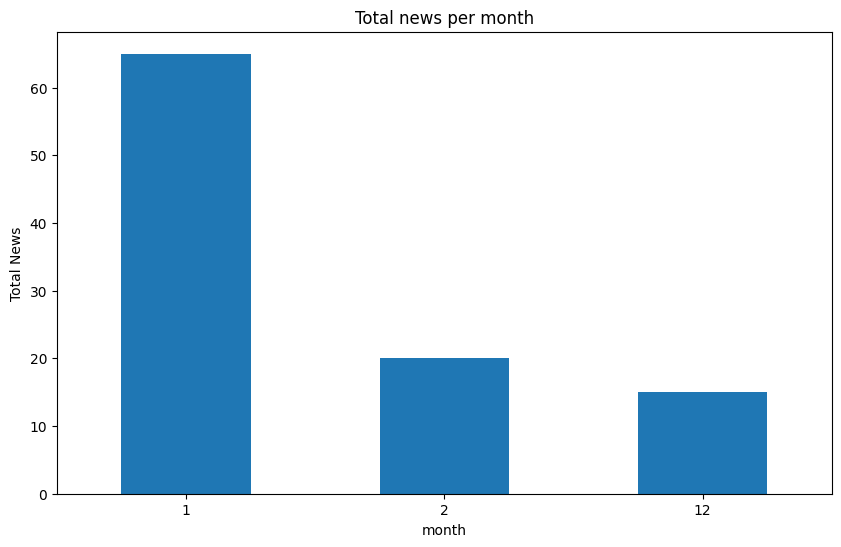
\includegraphics[width=0.45\textwidth]{figures/news_per_date.png}
    \caption{Total de noticias publicadas por mes.}
    \label{fig:eje2}
\end{figure}

\textbf{Nube de palabras más utilizadas:}

\begin{figure}[!ht]
    \centering
    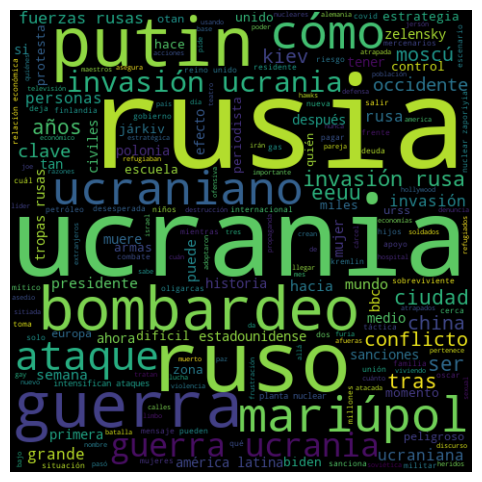
\includegraphics[width=0.45\textwidth]{figures/wordcloud.png}
    \caption{Word cloud.}
    \label{fig:eje2_1}
\end{figure}

\textbf{Distribución de los 10 bigramas y trigramas más frecuente:}

\begin{figure}[!ht]
    \centering
    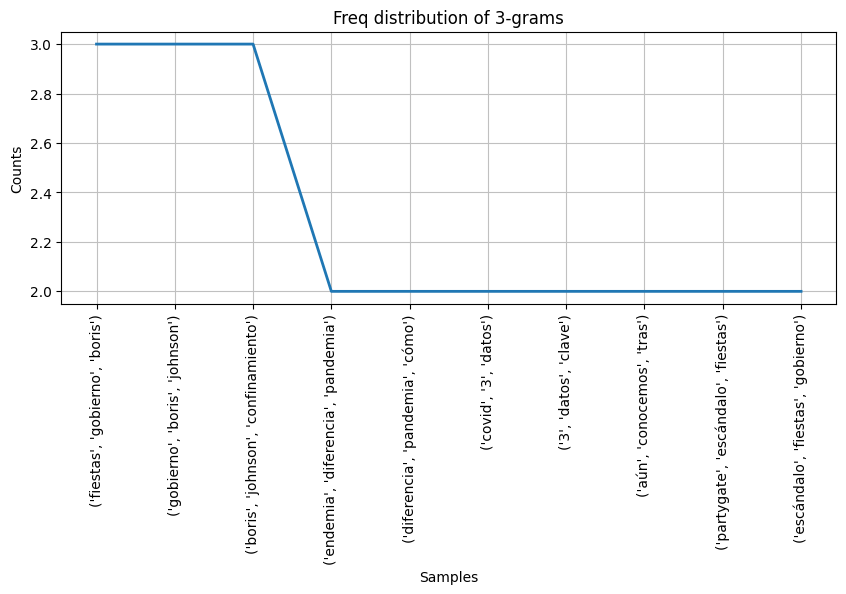
\includegraphics[width=0.45\textwidth]{figures/top_10_3grams_dist.png}
    \caption{Distribución de frecuencia de los 10 primeros trigramas.}
    \label{fig:eje2_2}
\end{figure} 

\newpage
\textbf{(Estudiante Mariana Guerrero Benavides-200173479)}

Con ayuda de las siguientes referencias: \cite{ChatGPT_scrapingScript} \cite{Scraping_web} Utilizando la fuente base de \cite{Usable_link} BBC Mundo \\
\textbf{Anexo Código}
\begin{lstlisting}[language=Python]
import json
import pandas as pd
from datetime import datetime
import seaborn as sns
import matplotlib.pyplot as plt
from bs4 import BeautifulSoup
import nltk
from nltk.corpus import stopwords
from nltk.util import ngrams
from wordcloud import WordCloud
from collections import Counter
import requests
import random

# Función para extraer datos de una pag web específica
def scrape_pag(soup, titulares): # BeautifulSoup para analizar y extraer datos del HTML
  # Toma el <script> del tipo de archivo
  script_tag = soup.find('script', string=lambda x: x and 'window.SIMORGH_DATA' in x)
  # Se extraen los datos del <script>
  json_data = script_tag.string
  # Se limpia el contenido para validarlo
  json_data = json_data.split('=', 1)[1].strip()
  # Parsea el archivo
  data = json.loads(json_data)
  # Accede a la clase que contiene datos de noticias
  curations = data['pageData']['curations']
  # Itera sobre los datos de la clase. Extrae los titulares y fechas
  for curation in curations:
    for summ in curation['summaries']:
      titulo = summ['title']
      fecha = summ['firstPublished']
      titulares.append({
          'Fecha': fecha,
          'Título': titulo
      })

# Url de la página a scrapear
pag_web = 'https://www.bbc.com/mundo/topics/c7zp57yyz25t'
pag = requests.get(pag_web) # Se realiza la solicitud a la página
soup = BeautifulSoup(pag.text, 'html.parser') # Parsea la página
titulares = [] # Inicializa la lista de titulares
scrape_pag(soup, titulares) # Scrapea la página inicial
# Toma el siguiente elemento del html
next_pag = soup.find('li', class_='next')
# Scrapear siguiente página
while next_pag is not None:
  next_pag_relativa = next_pag.find('a', href=True)['href']
  pag = requests.get(pag_web + next_pag_relativa)
  soup = BeautifulSoup(pag.text, 'html.parser')
  scrape_pag(soup, titulares)
  next_pag = soup.find('li', class_='next')

# Se crea un dataframe y se almacenan los datos extraídos
df = pd.DataFrame(titulares)
# Se guarda df en csv
df.to_csv('titulares.csv', index=False, encoding='utf-8') # exportación a csv

# Cádenas de Markov: 30 titulares aleatorios de los titulares existentes
def tokeniza_titulares(df): #Tokenización titulares
  tok = []
  for titular in df['Título']:
      titulares_tok = titular.split()
      tok.extend(titulares_tok)
  return tok

titulares_token = tokeniza_titulares(df) # Tokenización palabras de titulares

# Convertir el texto anterior a una lista donde se escojan terminos aleatorios
def texto_random(palabras, longitud_deseada=24):
  random.shuffle(palabras) # Mezcla los tokens
  generado = " ".join(palabras[:longitud_deseada])  #Combina los tokens
  return generado

# Se generan los titulares aleatorios
num_titulares_random = 30
for i in range(num_titulares_random):
  nuevos_titulares = texto_random(titulares_token, longitud_deseada=24)
  print(f"{i + 1}: {nuevos_titulares}")
print("-"*90)

nltk.download('stopwords') # descarga de las soptowords
stop_palabras = set(stopwords.words("spanish")) # se obtiene el conjunto de palabras vacías 

# Limpia y tokenización de las palabras: Función que divide los enunciados en palabras y elimina las palabras vacías.
def tokeniza_limpia(text):
  palabras = text.lower().split()
  limpiado = [word for word in palabras if word.isalpha() and word not in stop_palabras]
  return limpiado

todas_palabras = [word for titulo in titulares for word in tokeniza_limpia(titulo['Título'])]
cont_palabras = Counter(todas_palabras) # usado para contar la frecuencia de las palabras limpias.

# Genera las 10 palabras más usadas en enunciados
top_palabras = cont_palabras.most_common(10)
print(" \n Distribución de frecuencia de las palabras más utilizadas en todos los enunciados:")
print(top_palabras)
print("-"*90)

# Palabras más usadas por fecha de publicación
cont_dia = df.groupby("Fecha")["Título"].apply(lambda x: " ".join(x)).reset_index() # agrupa los datos por fecha y concatena los enunciados por estas
cont_dia["Titular_limpio"] = cont_dia["Título"].apply(tokeniza_limpia)
cont_dia["Palabra_comun"] = cont_dia["Titular_limpio"].apply(lambda x: Counter(x).most_common(1))
buscar_dia = "2023-10-04" # modificar fecha a elección
df["Fecha"] = pd.to_datetime(df["Fecha"]) # Pasamos la columna de fecha a objetos de fecha y hora de Pandas 
buscar_dia = datetime.strptime(buscar_dia, "%Y-%m-%d") 
buscar_año = buscar_dia.year # Se toma año y mes de lo que se busca
buscar_mes = buscar_dia.month
buscar_titular = df[df["Fecha"].apply(lambda x: x.year == buscar_año and x.month == buscar_mes)] # Filtro de titulares por año y mes
if not buscar_titular.empty:
  palabra_comun = Counter(" ".join(buscar_titular["Título"]).split()).most_common(10)
  print(f"Palabra más usada por fecha de publicación de la noticia: Se escogió la fecha {buscar_dia}:")
  print(palabra_comun)
else:
  print(f"No se encontraron palabras para la fecha {buscar_dia}")
print("-" * 90)

# Cantidad de artículos publicados por fecha
df["Fecha"] = pd.to_datetime(df["Fecha"])
df["Dia"] = df["Fecha"].dt.day # Extraer fecha por dia
articulo_dia = df["Dia"].value_counts().sort_index() # Cuenta el número de enunciados publicados por dia
# Gráfica de la cantidad de artículos publicados por fecha
plt.figure(figsize=(8, 5))
articulo_dia.plot(kind="bar")
plt.xlabel("Dia"), plt.ylabel("Cantidad de artículos")
plt.title("Cantidad de artículos publicados por fecha")
plt.show()
print("-"*90)

# Nube de las palabras más usadas
nube = WordCloud(width=800, height=400, background_color="white").generate(" ".join(todas_palabras))
plt.figure(figsize=(8, 5))
plt.imshow(nube, interpolation="bilinear")
plt.title("Nube de palabras más utilizadas")
plt.show()
print("-"*90)

# Distribución de los 10 bigramas y trigramas más frecuentes
def buscar_ngrams(texto, n):
  ngram_cont = Counter(ngrams(texto, n))
  return ngram_cont.most_common(10)

# Se encuentra los 10 más comunes bigramas y trigramas
bigramas = buscar_ngrams(todas_palabras, 2)
trigramas = buscar_ngrams(todas_palabras, 3)
# Gráfica de bigramas
niveles_bigrama, bigrama_cont = zip(*bigramas)
niveles_bigrama = [' '.join(label) for label in niveles_bigrama]
plt.figure(figsize=(8, 5))
plt.barh(range(10), bigrama_cont, tick_label = niveles_bigrama)
plt.xlabel('Frecuencia'), plt.ylabel('Bigramas')
plt.title('Distribución de los 10 bigramas más frecuentes')
plt.show()
# Gráfica de trigramas
niveles_trigrama, trigrama_cont = zip(*trigramas)
niveles_trigrama = [' '.join(label) for label in niveles_trigrama]
plt.figure(figsize=(8, 5))
plt.barh(range(10), trigrama_cont, tick_label = niveles_trigrama)
plt.xlabel('Frecuencia'), plt.ylabel('Trigramas')
plt.title('Distribución de los 10 trigramas más frecuentes')
plt.show()
\end{lstlisting}

\newpage 

\subsection{Explicación de los métodos implementados}
Primeramente se realiza el web scraping para extraer los datos de la página web ‘BBC NEWS MUNDO’ por medio de las librerías \underline{request} y \underline{BeautifulSoup}. Posteriormente, la librería Pandas para la manipulación y el manejo de los datos recolectados. 
\begin{itemize}
    \item El método pd.DataFrame() se utilizó para generar un dataframe a partir de los enunciados extraídos.  
    \item Para exportar esto datos a un archivo csv, se utiliza el método df.to\textunderscore csv(), guardándolo como ‘titulares.csv’. En este, se hace énfasis en que los índices de la fila no se incluyan en el archivo. 
    \item Para normalizar el texto (eliminar signos de puntuación y/o caracteres especiales), se utilizó la función download() de     NLTK para descargar los \textit{stopwords}, que, son palabras que ayudan a dar estructura al contenido, más no generan un aporte significativo en el texto. Al eliminarlas, se reduce la complejidad del texto, puesto que, estas suelen repetirse constantemente. Esta limpieza, se realizó mediante el método tokeniza\textunderscore limpia(), que devuelve una lista de palabras limpias.
    \item La función counter() de la librería collections se utilizó para poder contar la frecuencia de las palabras luego de haber tokenizado el contenido. Estas se guardan en un diccionario. 
    \item Para generar los 30 titulares aleatorios se hizo uso de las cádenas de markov, por medio del método texto\textunderscore random().
    \item De la librería Pandas se utilizó el método df.groupby(), en el cual agrupamos los datos en función de la columna ‘Fecha’. Al utilizar apply() se concatenan los titulares en un grupo de fecha. 
    \item Se utilizó pd.to\textunderscore datetime() para poder convertir la columna ‘Fecha’ a objetos de fecha y hora de Pandas, para permitir su análisis de manera más accesible. 
    \item Para contar los valores de la columna ‘Dia’ se utilizó el método value\textunderscore counts(), y se organizaron tales días de manera ascendente por medio del método sort\textunderscore index().
    \item Para la realización del diagrama de nubes, se utilizó el método generate() de la librería WordClouds de Python. Este permite generar tal diagrama, a partir de un \textit{text string}.
    \item Se utilizaron los n-gramas como técnica para el procesamiento del lenguaje natural, en donde podríamos obtener la serie de los $n$ términos (en este caso las palabras). En este caso, $n=2,3$ para la representación del bígama y trígrama respectivamente. 
\end{itemize}


\newpage

\section*{Entregable}

\begin{itemize}
    \item Archivo de Jupyter Notebook \texttt{.ipynb} con el código utilizado para generar las gráficas a partir del archivo \texttt{csv}.
     El archivo debe quedar de tal manera que si se cambia el \texttt{csv}, al ejecutar todas las celdas las gráficas se deben generar \textbf{todas} correctamente, así como también el \texttt{csv} con solo las columnas indicadas. Este punto es de vital importancia pues su código será probado con distintos archivos, con varias distribuciones de las probabilidades de las láminas.    \item Versión en PDF del informe,  el cual debe tener:
    \begin{itemize}
        \item Explicación de su código. 

        Deben explicar los métodos utilizados de las librerías \textbf{NumPy} y \textbf{Pandas}, para qué sirven de manera general y para qué les sirvieron en específico para la realización del trabajo.

        Además, es \textbf{obligatorio} el uso de la librería \textbf{Pandas} para la lectura y generación de los \texttt{csv} pedidos. 
    \end{itemize}
    \item Código fuente en \LaTeX  del informe.

    \item Los items listados deben ser enviados en forma separada. \textbf{NO} es necesario que adjunten los \texttt{csv} generados, pues su código debe ser capaz de generarlos.
\end{itemize}
